\section{Complexe Zahlen}
\subsection{Grundlagen}
\subsubsection{Imaginäre Einheit}
$j^2 = -1 \qquad e^{j\pi} = -1 \qquad \frac{1}{j} = -j$

\subsubsection{Darstellungsformen}
\begin{tabular}{ll}
	Cartesische Form: & $z = z_1 + j z_2$ \quad Wobei gilt: $z_1 = \text{Re}(z),
	\quad z_2 = \text{Im}(z)$ \\
	Polar Form: &   $z = r \cjs(\varphi) = r(\cos{\varphi} + j\sin{\varphi}) = r
	e^{j \varphi}$ 	\\
\end{tabular}
\subsubsection{Umrechnung}
\begin{tabular}{ll}
	Cartesisch $\rightarrow$ Polar: & $r = |z| = \sqrt{z_1^2 + z_2^2} \qquad   
		\varphi = arg(z) 
		        = 	\begin{cases} 
                       	\arctan(\frac{z_2}{z_1}) &z_1 \geq 0\\
                  		\arctan(\frac{z_2}{z_1}) + \pi &z_1 < 0
          			\end{cases}
          		=	\begin{cases}
          				\arccos(\frac{z_1}{r}) & z_2 \geq 0 \\
          				-\arccos(\frac{z_1}{r}) & z_2 < 0          		
          			\end{cases}$ \\
          			
	Polar $\rightarrow$ Cartesisch: & $z_1 = r \cdot cos(\varphi) \qquad z_2 = r
	\cdot sin(\varphi)$ \\
\end{tabular}


\subsection{Rechenregeln}
\begin{center}
\begin{tabular}{|l|l|l|}
	\hline
	\textbf{Operation} & \textbf{Cartesisch} & \textbf{Polar} \\
	\hline
	
	Addition \& Subtraktion & 
	\multicolumn{2}{|c|}{Selbige Regeln wie für
	$\mathbb{R}$}\\
	\hline
	
	Multiplikation ($a \cdot b$) &
	$ = (a_1 + j a_2) \cdot (b_1 + j b_2) = (a_1 b_1 - a_2 b_2) + j(a_1 b_2 + a_2
	b_1) $ &
	$ = r_a r_b \cjs(\alpha + \beta) = r_a r_b e^{j(\alpha +
	\beta)}$\\
	\hline 
	
	Division ($\frac{a}{b}$) &
	$ = \frac{a \cdot \overline{b}}{b \cdot \overline{b}}
	  = \frac{a_1 b_1 + a_2 b_2}{b_1^2 + b_2^2} + j \frac{a_2 b_1 - a_1
	  b_2}{b_1^2 + b_2^2}$ & 
	$ = \frac{r_a}{r_b} \cjs(\alpha - \beta) 
	  = \frac{r_a}{r_b} e^{j(\alpha - \beta)}$ \\
	\hline
	\hline
	
	\textbf{Operation} & \multicolumn{2}{|c|}{
		\textbf{Cartesisch}
	} \\
	
	\hline
	Conjugiert Complex $\overline{z}$ &
	\multicolumn{2}{|l|}{
		$ = \overline{z_1 + jz_2} = z_1 - jz_2 \qquad
		  z \cdot \overline{z} = |z|^2 = z_1^2 + z_2^2$
	} \\
	\hline
	\hline
	
	\textbf{Operation} & \multicolumn{2}{|c|}{
		\textbf{Polar}
	} \\
	
	\hline
	Wurzeln $\sqrt[n]{a}$ &
	\multicolumn{2}{|l|}{
		$ = \sqrt[n]{r_a} \cjs(\frac{\varphi}{n}+k\frac{2\pi}{n}) 
		  = \sqrt[n]{r_a} e^{j(\frac{\varphi}{n} + k \frac{2\pi}{n})} \quad 
		  (k = 0, 1, \ldots, n-1 \Rightarrow \text{n Lösungen in } \mathbb{C} !)
		$
	} \\
	\hline
	
	Potenzen $a^n$ &
	\multicolumn{2}{|l|}{
		$ = r_a^n \cjs(n\varphi) 
		  = r_a^n e^{jn\varphi}
		$
	} \\
	\hline
	
	$e^z$ &
	\multicolumn{2}{|l|}{
		$ e^{z_1+jz_2} 
		  = e^{z_1} \cjs(z_2) 
		  = e^{z_1} (\cos{z_2} + j\sin{z_2})
		$
	} \\
	\hline
	
	Moivre'sche Formel &
	\multicolumn{2}{|l|}{
		$ \text{cjs}^n(\varphi) 
		  = (\cos{\varphi} + j\sin{\varphi})^n 
		  = \cos(n\varphi) +j\sin(n\varphi) \quad (n \in \mathbb{N})
		$
	} \\
	\hline
	
	Logarithmus $Ln(a)$ &
	\multicolumn{2}{|l|}{
		$ = \ln{r_a} + j (\varphi + 2k \pi)$
	} \\
	\hline
\end{tabular}
\end{center}

\textbf{Bemerkungen:}
\begin{itemize}
    \item Allgemeine Potenzen $a^b,\;a,b \in \mathbb{C}$ können mit $e^{b \cdot 
    	Ln(a)}$ und den bekannten für $\mathbb{R}$ gültigen Potenzregeln gelöst
    	werden.
    \item Re$\left (\frac{a}{b} \right) = 0$: Die beiden compl. Zahlen $a, b$
    	stehen senkrecht zueinander.
\end{itemize}


\subsection{Einheitswurzeln}
\begin{tabular}{p{10cm}p{8cm}}
\begin{itemize}
  \item Einheitswurzeln treten als reelle Zahlen $1$ bzw. $\mp 1$ oder dann als
  konjugiert komplexe Zahlenpaare auf.
  \item Die Einheitswurzeln können nach obigen Regeln berechnet werden, wobei $r
  = 1$ ist. 
  \item Berechnung: 
  		$ \sqrt[n]{e} = \sqrt[n]{1} = \cjs(k \frac{2\pi}{n}) 
		  = e^{j(k \frac{2\pi}{n})} $  \newline
		$  (k = 0, 1, \ldots, n-1 \Rightarrow \text{n Lösungen in } \mathbb{C} !)$
\end{itemize} 
&
\begin{center}
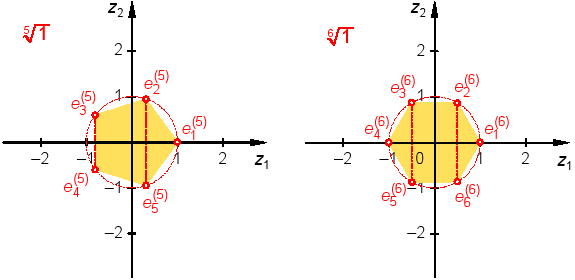
\includegraphics[width=7cm]{./bilder/einheitswurzel.png}
\end{center} \\
\end{tabular}

\textbf{12.Einheitswurzel:} \\
\begin{tabular}{llllll}
	$e^{(12)}_1 = 1$ & $e^{(12)}_2 = \frac{\sqrt3}{2} + \frac12j$ & $e^{(12)}_3 =
	\frac12 + \frac{\sqrt3}{2}j$ & $e^{(12)}_4 = j$ & $e^{(12)}_5 = -\frac12 +
	\frac{\sqrt3}{2}j$ & $e^{(12)}_6 = -\frac{\sqrt3}{2} + \frac12 j$ \\
	$e^{(12)}_7 = -1$ & $e^{(12)}_8 = -\frac{\sqrt3}{2} - \frac12 j$ &
	$e^{(12)}_9 = -\frac12 - \frac{\sqrt3}{2}j$ & $e^{(12)}_{10} = -j$ &
	$e^{(12)}_{11} = \frac12 - \frac{\sqrt3}{2}j$ & $e^{(12)}_{12} =
	\frac{\sqrt3}{2} - \frac12j$ \\
\end{tabular}



\subsection{Nullstellen von Polynomen}
\begin{itemize}
  \item Ein komplexes Polynom p(z) vom Grad $n$ hat in $ \mathbb{C}$ genau $n$
  Nullstellen.
  \item Alle Nullstellen liegen in einer Kreisscheibe um den Ursprung mit dem
  Radius $ \sum\limits_{k=0}^{n} \left| \frac{a_k}{a_n} \right|$
  \item Bei Polynomen mit reellen Koeffizienten treten nicht-reelle Nullstellen
  immer als conj.-compl. Paare ($z_0$ und $\overline{z_0}$) auf.
  \item Berechnung: Nullstellen abspalten , 2. Grades: Mitternachtsformel (siehe
  Kapitel \ref{Diverses}) 
\end{itemize}

\subsection{Überlagerung von harmonischen Schwingungen}
$$A \cdot \sin(\omega t + \varphi) = Im[A \cdot e^{j(\omega t + \varphi)}] =
Im[\underbrace{A \cdot e^{j\varphi}}_{\text{\tiny{Complexe Amplitude}}}
\cdot \underbrace{e^{j\omega t}}_{\text{\tiny{Zeitfunktion}}}]$$
%
%Alle komplexen Schwingungen in kartesische Form umwandeln und addieren, danach
%wieder zurück in Polarform $ A_{total} \cdot e^{j\varphi}$ zurückwandeln.
%
$$ A_1 \cdot \sin(\omega t + \varphi_1) + A_2 \cdot \cos(\omega t + \varphi_2) 
 \quad \Rightarrow \quad 
 Im[A_1 \cdot e^{j(\omega t + \varphi_1)} + A_2 \cdot e^{j (\omega t + \varphi_2
 + \frac{\pi}{2})}] \quad \Rightarrow \quad 
 Im[e^{j \omega t} \cdot  (A_1 \cdot e^{j \varphi_1} + A_2 \cdot e^{j (\varphi_2
 + \frac{\pi}{2})}]$$ 
Complexe Amplituden in cartesische Form umwandeln, zusammenzählen und wieder
zurück in Polarform wandeln.
$$ Im[e^{j \omega t} \cdot  (A_{total} \cdot e^{j \varphi_{total}})] 
 \quad \Rightarrow \quad 
 Im[A_{total} \cdot e^{j (\omega t + \varphi_{total})}] 
 \quad \Rightarrow \quad 
 A_{total} \cdot \sin(\omega t + \varphi_{total})$$

%Bsp: 
%$y = y_1 + y_2 = A_1 \sin(\omega t + \varphi_1) + A_2 \underbrace{\cos(\omega t
%+ \varphi_2)}_{\text{\tiny{zu sin verwandeln}}}
%= A_1 \sin(\omega t + \varphi_1) - A_2 \sin(\omega t + (\varphi_2
%-\frac{\pi}{2}))$\\
%$= \text{Im}(\underbrace{A_1 e^{j\varphi_1}}_{\text{\tiny{$A_{1im} = A_1 \cjs
%A_1 \cdot \sin(\omega t + \varphi_1) + \varphi_1$}}} e^{j\omega t} - 
%\underbrace{A_2 e^{j(\varphi_2 - \frac{\pi}{2})}}_{\text{\tiny{$A_{2im} = A_2 \cjs
%(\varphi_2 - \frac{\pi}{2})$}}} e^{j \omega t}) 
%= (A_{1im} + A_{2im}) \sin(\omega t)$